

\begin{frame}{Beviser}
    1. Hva vet vi?\\
    
    2. Hva beviser vi? \\
    
    3. Kan vi knytte det sammen?\\
    
    (4. Kan vi skrive det som formler eller kan vi tegne noe?)\\

    (5. Skriv ned hva dere prøve å bevise!) %raus?
\end{frame}

%\begin{frame}{Beviser eksempel}
    %en for formler og en for tegner? Mengde? En av dem er nok?
%\end{frame}

\begin{frame}{Direkte bevis}
    Et direkte bevis for $p \rightarrow q$ er et som antar at $p$ = T, og viser at det medfører at $q$ = T.\\
    Dette er ofte de enkleste bevisene. Hvis du har formler du bare må knytte sammen, forsøk det først.\\
    
    \pause
    \begin{block}{Vis at om $x$ og $y$ er oddetall, da er $x + y$ et partall.}
        Vi tar to oddetall $x$ og $y$. Da kan vi omskrive dem:\\
        $x = 2a+1$, $y = 2b+1$, for $a, b \in \mathbb{N}_0$.\\
        Nå viser vi at summen er partall: $x+y=2c$, $c \in \mathbb{N}_0$\\
        Da er $x + y = (2a+1) + (2b+1) = 2a + 2b + 2 = 2(a+b+1)$.\\
        Siden vi ganger med $2$ blir $2(a + b + 1)$ et partall uavhengig av hva $a + b + 1$ er.\\
        \qed
    \end{block}
\end{frame}

\begin{frame}{Kontrapositivt bevis (/proof by contraposition)}
    Istedet for å bevise $p \rightarrow q$, er det ofte lettere å bevise $\lnot q \rightarrow \lnot p$. De uttrykkene er helt ekvivalente.\\
    Det vil si å anta at $\lnot q = F$, og vise at da må også $\lnot p = F$.\\
    
    \pause
    \begin{block}{For ethvert heltall n har vi at hvis $n^2$ er et partall, så er n også et partall.}
        $n^2=2k \rightarrow n=2l$;    $k,l\in\mathbb{N}$\\
    \pause
        $n=2l+1 \rightarrow n^2=2k+1$\\
        $(n)^2=(2l+1)^2=4l^2+4l+1=2(2l^2+2l)+1=2k+1$ hvor $k=2l^2+2l \in\mathbb{N}$\\
    \pause
        $\implies$ hvis $n$ IKKE er et partall så er heller ikke $n^2$ et partall.\\
        $\implies$ hvis $n^2$ er et partall så er også $n$ et partall.
        \qed
    \end{block}
\end{frame}

\begin{frame}{Motsigelsesbevis (/proof by contradiction)}
    For å bevise en proposisjon $p$, kan det vi heller bevise at $\lnot p$ leder til en motsigelse. Det vil si, motbevis det motsatte.
    
    \pause
    \begin{block}{Vis at summen av et rasjonalt tall $\frac{a}{b}$ og et irrasjonalt tall $c$ også er et irrasjonalt tall.}
    Vi antar det motsatte: at summen blir et rasjonalt tall: $\frac{a}{b}$ + $c$ = $\frac{e}{d}$ for $e, d \in \mathbb{Z}$.\\
    $\implies \frac{e}{d} - \frac{a}{b} = c$\\
    $\implies \frac{b\cdot d - a \cdot d}{b\cdot d} = c$\\
    Men det impliserer at $c$ er et rasjonalt tall. [motsigelse!]\\
    Derfor er det usant at summen er et rasjonalt tall\\
    $\implies$ summen må være irrasjonal
    \qed
    
    \end{block}
\end{frame}

\begin{frame}{Uttømmende bevis (/proof by exhaustion)}
    OBS! Ingen garanti for å få poeng! Men hvis du har god tid og ingen bedre ideer, prøv det. Noen ganger greier vi ikke finne på et elegant bevis. Da tar vi heller for oss hvert enkelt tilfelle hver for seg, og når vi har vist at det holder for absolutt alle tilfeller har vi bevist påstanden. Merk at da må det være et endelig antall tilfeller.
    \pause
    \begin{block}{Vis at alle sommer-OL har blitt arrangert i årstall delelige på 4.}
        \pause
        1896 mod 4 = 0 \checkmark \\
        1900 mod 4 = 0 \checkmark \\
        %1904 mod 4 = 0 \checkmark \\
        {[... de neste 29 linjene er trivielle og etterlatt som en oppgave for leseren ...]}\\
        2020 mod 4 = 0 \checkmark
    \end{block}
    \pause
    Dette er altså ikke et komplett bevis. Vi må faktisk vise alle tilfeller før vi er ferdig.
\end{frame}

\begin{frame}{Motbevis}
    For å bevise at en påstand er usann, holder det vanligvis bare å finne et moteksempel. Dette er vanligvis den letteste typen bevis.\\
    OBS! Det er det eneste øyeblikket hvor det er ok å stoppe etter et eksempel.
    \pause
    \begin{block}{Påstand: det er ikke mulig å plassere 8 dronninger på et sjakkbrett uten at noen av dem truer hverandre.}
    \pause
    \begin{figure}
        \centering
        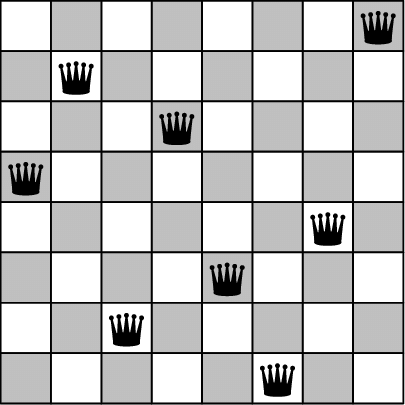
\includegraphics[scale=0.20]{images/8 queens.png}
        % \caption{Motbevis}
        \label{fig:my_label}
    \end{figure}
    
    \end{block}
\end{frame}

